\documentclass{article}
\usepackage{amsmath}
\usepackage{tikz}
\usetikzlibrary{arrows.meta, calc, positioning}

\begin{document}

\begin{figure}[h]
    \centering
    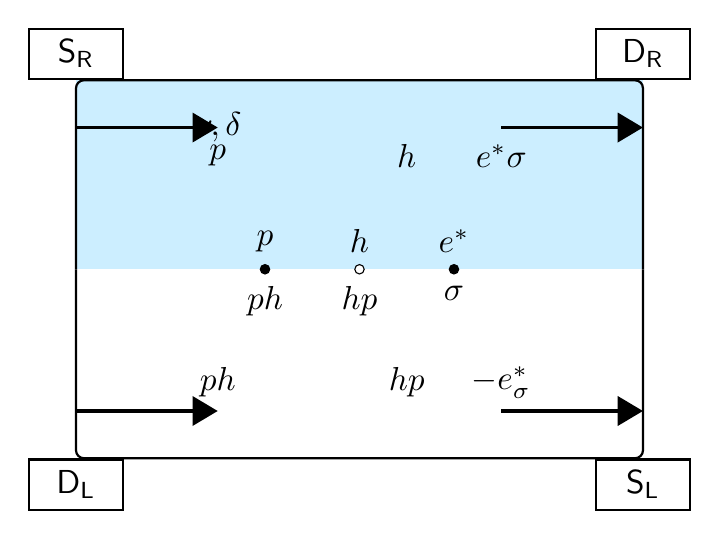
\begin{tikzpicture}[scale=1.2, every node/.style={transform shape}]
        % Define colors
        \definecolor{lightblue}{RGB}{204, 238, 255}
        
        % Draw the shaded area
        \fill[lightblue] (-3,0) rectangle (3,2);
        
        % Draw the top and bottom edges
        \draw[thick, rounded corners=1mm] (-3,0) -- (-3,-2) -- (3,-2) -- (3,0);
        
        % Draw the left and right boundaries
        \draw[thick, rounded corners=1mm] (-3,0) -- (-3,2) -- (3,2) -- (3,0);
        
        % Draw the labels for the boundaries
        \node at (-3,2) [draw, thick, minimum width=1cm, minimum height=0.5cm, anchor=south] {$\mathsf{S_R}$};
        \node at (3,2) [draw, thick, minimum width=1cm, minimum height=0.5cm, anchor=south] {$\mathsf{D_R}$};
        \node at (-3,-2) [draw, thick, minimum width=1cm, minimum height=0.5cm, anchor=north] {$\mathsf{D_L}$};
        \node at (3,-2) [draw, thick, minimum width=1cm, minimum height=0.5cm, anchor=north] {$\mathsf{S_L}$};
        
        % Draw the arrows
        \draw[-{Triangle[scale=1.5]}, very thick] (-3,1.5) -- (-1.5,1.5);
        \draw[-{Triangle[scale=1.5]}, very thick] (1.5,1.5) -- (3,1.5);
        \draw[-{Triangle[scale=1.5]}, very thick] (-3,-1.5) -- (-1.5,-1.5);
        \draw[-{Triangle[scale=1.5]}, very thick] (1.5,-1.5) -- (3,-1.5);
        
        % Draw the circles and labels
        \node[circle, draw, fill=black, inner sep=1pt, label=above:$p$, label=below:$ph$] at (-1,0) {};
        \node[circle, draw, fill=white, inner sep=1pt, label=above:$h$, label=below:$hp$] at (0,0) {};
        \node[circle, draw, fill=black, inner sep=1pt, label=above:$e^*$, label=below:$\sigma$] at (1,0) {};
        
        % Draw the labels for the processes
        \node at (-1.5,1.2) {$p$};
        \node at (-1.5,-1.2) {$ph$};
        \node at (0.5,1.2) {$h$};
        \node at (0.5,-1.2) {$hp$};
        \node at (1.5,1.2) {$e^*\sigma$};
        \node at (1.5,-1.2) {$-e^*_\sigma$};
        
        % Draw the labels for the charges
        \node at (-1.5,1.5) {$\nu,\delta$};
        
    \end{tikzpicture}
    \caption{Four possible tunneling processes between the top and bottom edges of a non-Abelian state (shaded area). All processes result in transferring an anyon charge $e^*=e/4$ from top to bottom (straight arrow), however, the entropy transfer is different in each process. For example, in the non-Abelian $\nu=5/2$ state, the $p$ process transfers a quasiparticle with charge $e^*$ together with its internal entropy $s_\sigma =\log(\sqrt{2})$ from top to bottom. The $ph$ process has an identical charge transfer, but it takes entropy from both the top and the bottom edges and heats the bulk. The $hp$ and the $h$ processes are similar and are discussed in the text.}
    \label{fig:tunneling_processes}
\end{figure}

\end{document}